\documentclass{article}
\usepackage{graphicx}
\usepackage{color}
\graphicspath{ {/asay/Desktop/images/} }
\usepackage{xepersian}


\title{پاسخ تمرین شماره۴ درس معماری کامپیوتر}
\author{امیر حسین عاصم یوسفی \\ ۹۶۱۱۰۳۲۳}
\settextfont{B Nazanin}

\begin{document}
	\maketitle
	\section*{سوال ۱  : }
	\subsection*{\textcolor{red}{الف}}
	برای این قسمت جدول به شکل زیر می باشد  : 
	\begin{center}
	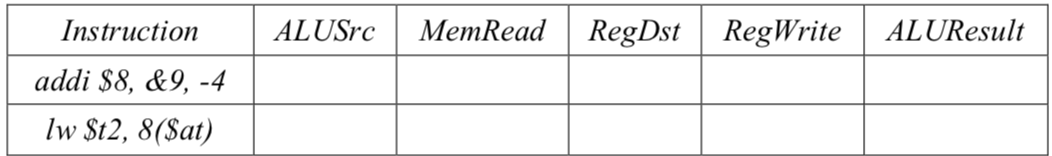
\includegraphics[width=1\textwidth]{table1}
	\end{center}

\subsection*{\textcolor{red}{ب}}
با توجه به این که  ساختار دستورات 
\lr{I type }
به صورت زیر می باشد  : 
	\begin{center}
	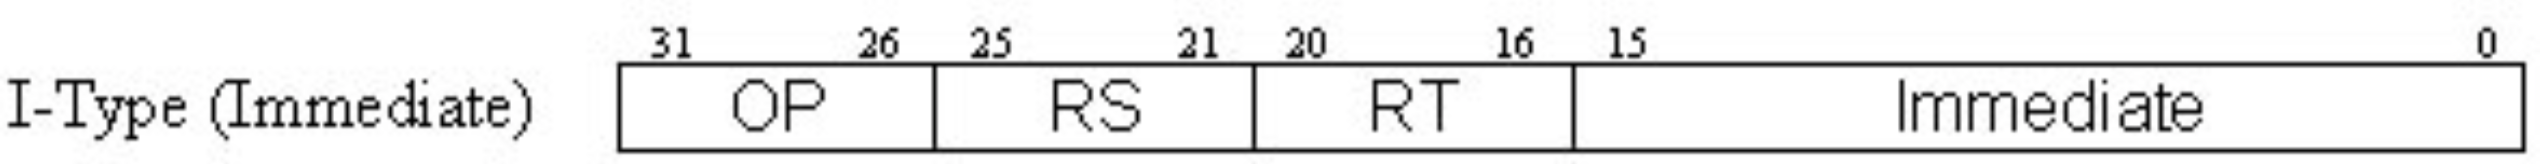
\includegraphics[width=1\textwidth]{itype}
\end{center}
در صورتی که خطای کفته شده اتفاق بیافتد همیشه مقدار آدرس رجیستر مقصد را از بیت های ۱۱ تا ۱۵ می خواند که با توجه به شکل بالا این مقدار نامعتبر می باشد زیرا ۱۵ بیت اول نشان دهنده مقدار 
\lr{immediate }
می باشد و آدرس رجیستر داخل آن قرار ندارد بنابراین این دستور دیگر به  درستی انجام نمی شود  . 
\hrule
\section*{سوال ۲  : }
\subsection*{\textcolor{red}{الف}}
این دستور دستور 
\lr{\textcolor{red}{beq}}
می باشد  . و علت استفاده از این بخش محاسبه کردن آدرس دستور بعدی می باشد اما با توجه به قرمول زیر 
\begin{center}
	$PC  = PC + 4 + (offset <<2 )$
\end{center}
\subsection*{\textcolor{red}{ب}}
زمانی که 
\lr{PC}
را با ۴ جمع می کنیم در واقع ۴ بیت بالایی آدرس دستور بعدی مشخص می شود ولی چون آدرس بعدی در این نوع دستورات طبق فرمول گفته شده می باشد بنابراین باید ۲۸ بیت پایین 
\lr{PC}
را با 
\lr{offset<<2}
پر کنیم و چون 
\lr{offset}
۲۶ بیت دارد با دو بار شیفت دادن به سمت چپ و تبدیل کردن آن به ۲۸ بیت آن را به جای ۲۸ بیت پایینی 
\lr{PC}
قرار می دهیم تا به این ترتیب ۳۲ بیت آدرس دستور بعدی محاسبه شود. 
\subsection*{\textcolor{red}{پ}}
 سیگنال 
\lr{ZERO}
زمانی یک می شود که مقدار موجود در دو رجیستر با یک دیگر برابر باشد و زمانی صفر می شود که مقدار موجود در دو رجیستر با یک دیگر برابر نباشند بنابراین از این سیگنال برای شناسایی برابر بودن مقدار داخل دو رجیستر استفاده می شود  . 
\\
سیگنال کنترلی 
\lr{BRANCH}
برای کنترل کردن انجام عملیات از نوع
\lr{BRANCH}
یعنی 
\lr{ beq)}
و زمانی یک می شود که دستور ما به صورت پرش به یک دستور با شرایط باشد  .
\\
یکی از آن ها کافی 
\textcolor{red}{نیست}
زیرا اگر فقط سیگنال
\lr{ZERO}
داشته باشم آن گاه هر بار که مقدار داخل دو رجیستر با یک دیگر برابر باشد مقدار 
\lr{PC}
با
\lr{PC + 4 + (offset<<2)}
جایگزین می شود که این می تواند اجرای  دستورات مانند 
\lr{sub}
را دچار مشکل کند به این ترتیب که اگر دو عدد مساوی را از یکدیگر کم کنیم مقدار حاصل صفر می شود و به این ترتیب مقدار سیگنال 
‌\lr{ZERO}
برابر با یک می شود بنابراین دیگر پردازنده به دستور بعدی نمی رود و مقدار 
\lr{PC}
معتبر نخواهد بود . 
\\
از طرفی اگر فقط سیگنال 
\lr{BRANCH}
داشته باشیم بازهم نمی توانیم هر بار که این سیگنال یک می شود بدون توجه به برابری مقدار داخل دو رجیستر پرش انجام می شود  . که این باعث درست اجرا نشد دستورات از نوع 
\lr{BRANCH}
میشود . 
\hrule
\section*{سوال ۳}
با توجه به این که ساختار دستورات 
\lr{J type}
به صورت زیر می باشد  : 
\begin{center}
	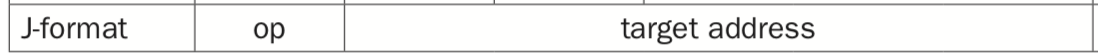
\includegraphics[width=1\textwidth]{jtype}
\end{center}
\subsection*{\textcolor{red}{\lr{jar}}}
برای این که این دستور انجام شود باید یک واحد شیفت دهنده که مقدار موجود در 
\lr{Instruction[25:0]}
را دو بیت به سمت چپ شیفت می دهند  .  در مر حله بعد آن را با مقدار 
\lr{PC+4}
که خروجی اولین 
\lr{adder}
می باشد ترکیب می کنیم به این صورت که خروجی واحد شیفت دهنده را در ۲۸ بیت پایینی 
\lr{PC}
قرار می دهیم و به این ترتیب آدرس پرش به دست می آید  . 
\\
در مرحله بعد باید یک سیگنال کنترلی به اسم 
\lr{Jump}
اضافه کنیم  . 
\\
در مرحله بعد باید یک مالتی پلکسر ۲ به ۱ قرار دهیم که سیگنال 
\lr{select}
آن همان سیگنال 
\lr{Jump}
میباشد و ورودی صفر آن ، خروجی مالتی پلکسری می باشد که سیگنال کنترلی 
\lr{PCSrc}
دارد . و ورودی یکم آن مقدار 
\lr{PC + 4 + (Instruction[25:0]<<2)}
می باشد . بنابراین شکل نهایتا به صورت زیر خواهد بود  : 
\begin{center}
	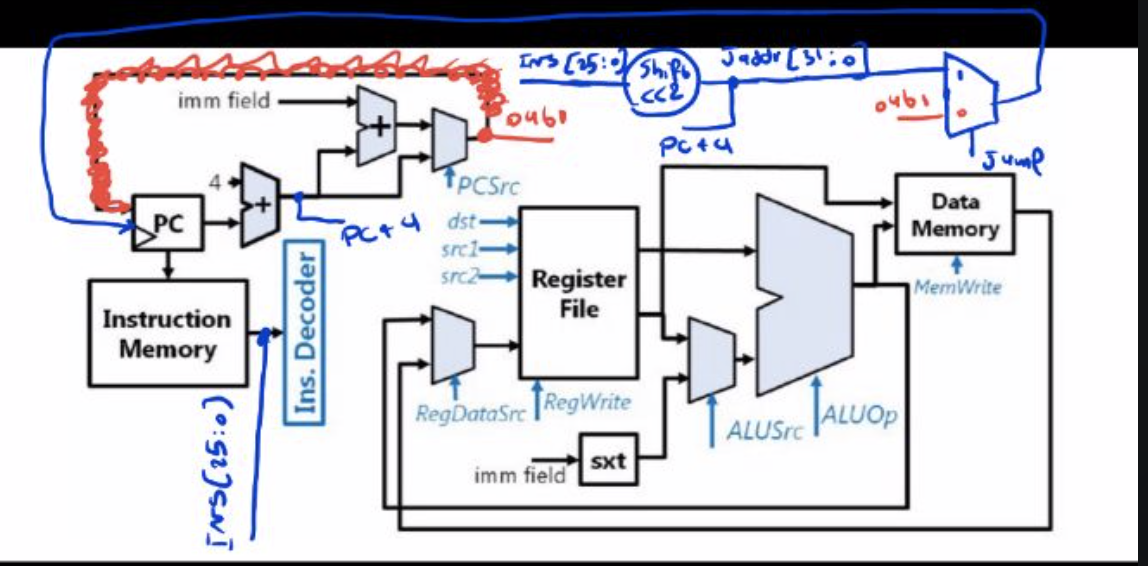
\includegraphics[width=1\textwidth]{jar}
\end{center}
\subsection*{\textcolor{red}{\lr{jal}}}
برای این دستور باید علاوه بر تغییرات بخش قبل ، مالتی پلکسری که سیگنال 
\lr{select }
آن 
\lr{RegDataSrc}
می باشد را از ۲ به یک ، به یک مالتی پلکسر ۳ به یک تغییر دهیم و در ورودی دوم آن مقدار 
\lr{PC+4}
را که خروجی 
\lr{adder}
اول می باشد را قرار دهیم و به سیگنال 
\lr{dst}
هم آدرس رجیستر مورد نظر برای کپی کردن را بدهیم 
\lr{(\$ra)}
بنابراین نهایتا شکل به صورت زیر در می آید  : 
\begin{center}
	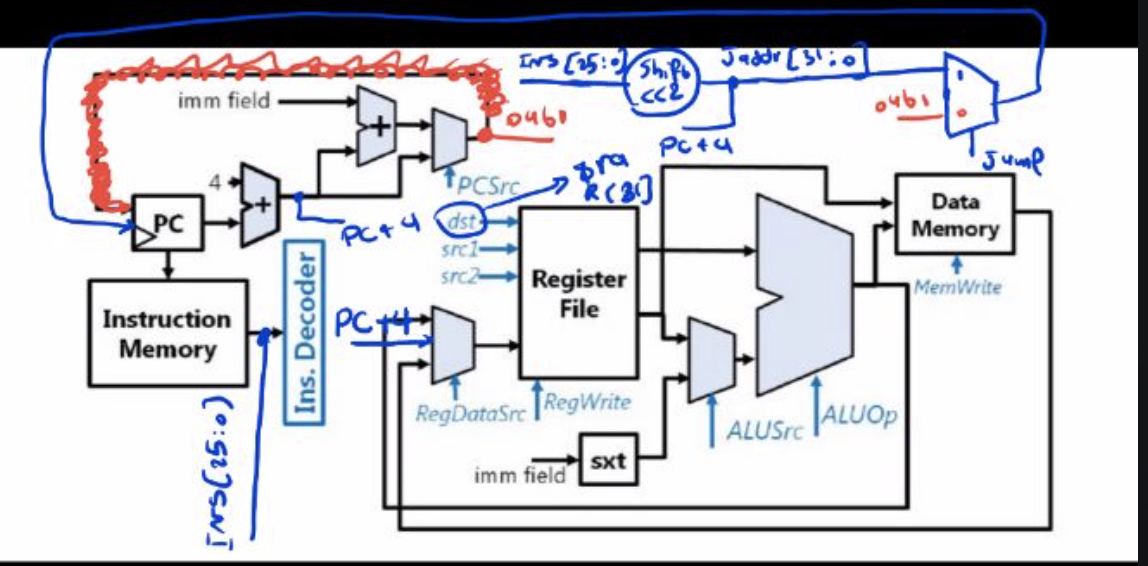
\includegraphics[width=1\textwidth]{jal}
\end{center}
\hrule
\section*{سوال ۴  }
\subsection*{\textcolor{red}{الف}}
این 
\lr{data path}
مربوط به یک دستور 
\lr{R type }
میباشد  . 
\subsection*{\textcolor{red}{ب}}
تاخیر این دستور برابر است با  : 
\begin{center}
	\lr{R type$_{delay}$  =  Instruction memory  + Registers  + ALU + Registers  = 2 + 1 + 2 + 1  = 6ns}

\end{center}
\subsection*{\textcolor{red}{ج}}
با توجه به این که معادلات زمانی به صورت زیر می باشد  : 
\begin{center}
	\lr{Minimum instruction delay  = d$_{min} $ + d $_{ff}$ > hold \_ time}
	\\
	\lr{Max instruction delay  + setup\_ time = d $_{max}$ + d$_{ff}$ + setup \_ time < clock }
\end{center}
اما برای سادگی می توان به جای 
\lr{ d$_{min} $ + d $_{ff}$ }
مقدار مینیمم تاخیر دستورات را درنظر گرفت . برای به دست آوردن این مقدار تاخیر تمام دستورات را به دست می آوریم  : 
\begin{center}
	\lr{delay $_{beq}$ = 2 + 1 + 2  = 5ns }
	\\
	\lr{delay $_{sw}  $ = 2 + 1 + 2  + 2 = 7ns}
	\\
	\lr{delay $_{lw} $= 2 + 1 + 2 + 2  +1 = 8ns}
\end{center}
بنابراین مینیمم تاخیر دستورات برابر با 
\lr{\textcolor{red}{5ns}}
می باشد بنابراین داریم 
\begin{center}
	\lr{hold \_ time  < 5ns}
\end{center}
هم چنین باز برای سادگی می توان 
\lr{d $_{max}$ + d$_{ff}$}
را ماکسیمم تاخیر دستورات در نظر گرفت  که برابر است با 
\lr{\textcolor{red}{8ns}}
بنابراین برای کلاک داریم  : 
\begin{center}
	\lr{8ns  + 0.3 ns  = 8.3ns}
	
\end{center}
بنابراین کران پایین برای کلاک برابر است با 
\lr{\textcolor{red}{8.3ns}}
\hrule
\section*{سوال ۵ }
\subsection*{\textcolor{red}{الف}}
برای این بخش باید توجه کرد که اگر این اشکال به وجود بیاید تنها دستورات 
\lr{beq}
و 
\lr{sw}
به درستی کار می کنند زیرا در دستور 
\lr{beq}
نه از واحدهای 
\lr{data memeory }
استفاده می کنیم و نه از واحد 
\lr{Registers}
بنابراین اشکال به وجود آمده هیچ ایرادی در اجرای این  دستور به وجود نمی آورد . 
\\
برای دستور 
\lr{sw}
چون آدرس رجیستر مقصد در بیت ها ۱۶ تا ۲۰ می باشد با همیشه صفر بودن سیگنال
\lr{RegDst}
هیچ اشکالی در اجرای این دستور به وجود نمی آید  . 
\subsection*{\textcolor{red}{ب}}
با توجه به این که میانگین اجرای دستورات برای این پردازنده به شکل زیر می باشد  : 
\begin{center}
	\lr{0.48 * 6ns + 0.22 * 8ns + 0.11 * 7ns + 0.19 * 5ns = 6.36ns}
\end{center}
بنابراین اگر بتوانیم سیگنال 
\lr{RegDst}
 را درست کنیم حجم بیشتری از دستورات که شامل دستورات 
 \lr{Arithmetic}
 میباشد را می توان پوشش داد که مقرون به صرفه تر است  . 
 \subsection*{\textcolor{red}{ج}}
 با توجه به این که فقط دو دستورات 
 \lr{R type}
 و دستور 
 \lr{lw}
 نیاز به سیگنال 
 \lr{MemtoReg}
 دارند و با توجه به مقدار سیگنال های کنترلی برای دستورات گفته شده که به صورت زیر می باشد  
 \begin{center}
 	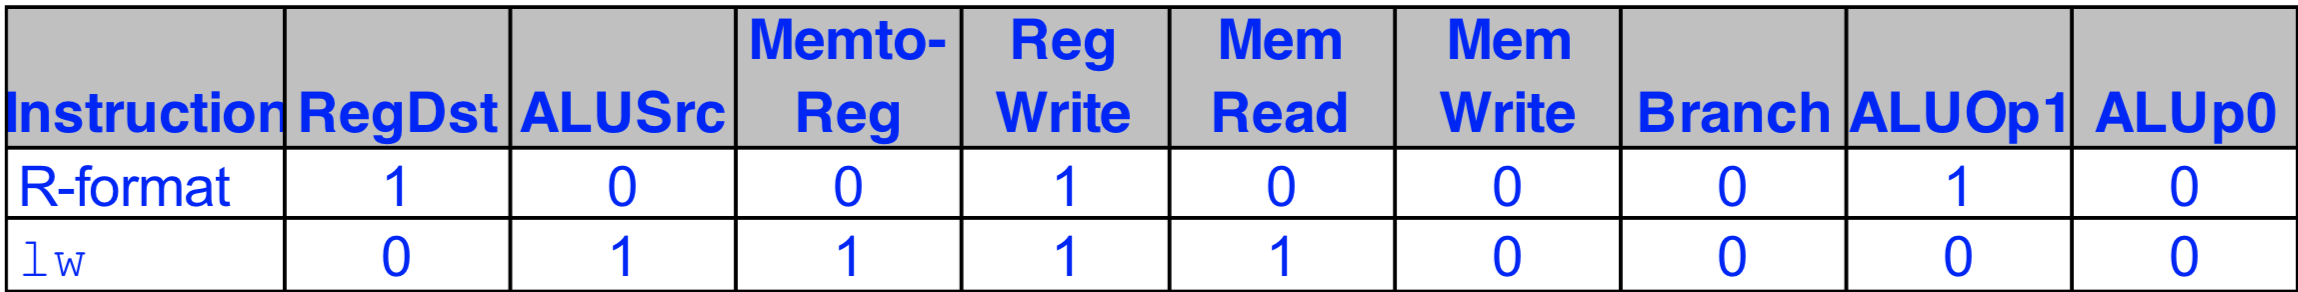
\includegraphics[width=1\textwidth]{table}
 \end{center}
 می توان دید که اگر مقدار دو سیگنال 
 \lr{RegWrite}
 و 
 \lr{MemRead}
را با یکدیگر 
\lr{and}
کنیم و مقدار سیگنال 
\lr{MemtoReg}
را از آن بگیریم می توانیم این اشکال را بر طرف کرد . 
\\
انتخاب این دو سیگنال به این دلیل است که اگر سیگنال 
\lr{RegWrite}
داشته باشیم و نوشتن در حافظه نداشته باشیم یعنی دستور از نوع 
\lr{R type}
است بنابراین باید مقدار سیگنال 
\lr{MemtoReg}
برابر با صفر باشد که برابر حاصل 
\lr{and}
این دو سیگنال است  . همچنین برای دستور این قانون صدق می کند . 
\hrule
\section*{سوال ۶}
باید مالتی پلکسری که سیگنال 
\lr{select}
آن 
\lr{MemtoReg}
و مالتی پلکسری که سیگنال 
\lr{select}
آن 
\lr{RegDst}
می باشد تبدیل به ماکس های ۳ به یک کنیم که برای ماکس اولی در ورودی دوم باید مقدار 
\lr{PC+4}
و برای ماکس دوم در ورودی دم آدرس رجیستر مقصد را می دهیم  .
\\
همچنین باید یک سیگنال کنترلی به نام 
\lr{\textcolor{red}{Jump}}
اضافه کنیم و هم چنین باید یک واحد شیفت دهنده به چپ برای محاسبه ۲۸ بیت پایین 
\lr{PC}
هم باید اضافه کنیم و با توجه به تغییرات بالا شکل نهایی به صورت زیر است  : 
 \begin{center}
	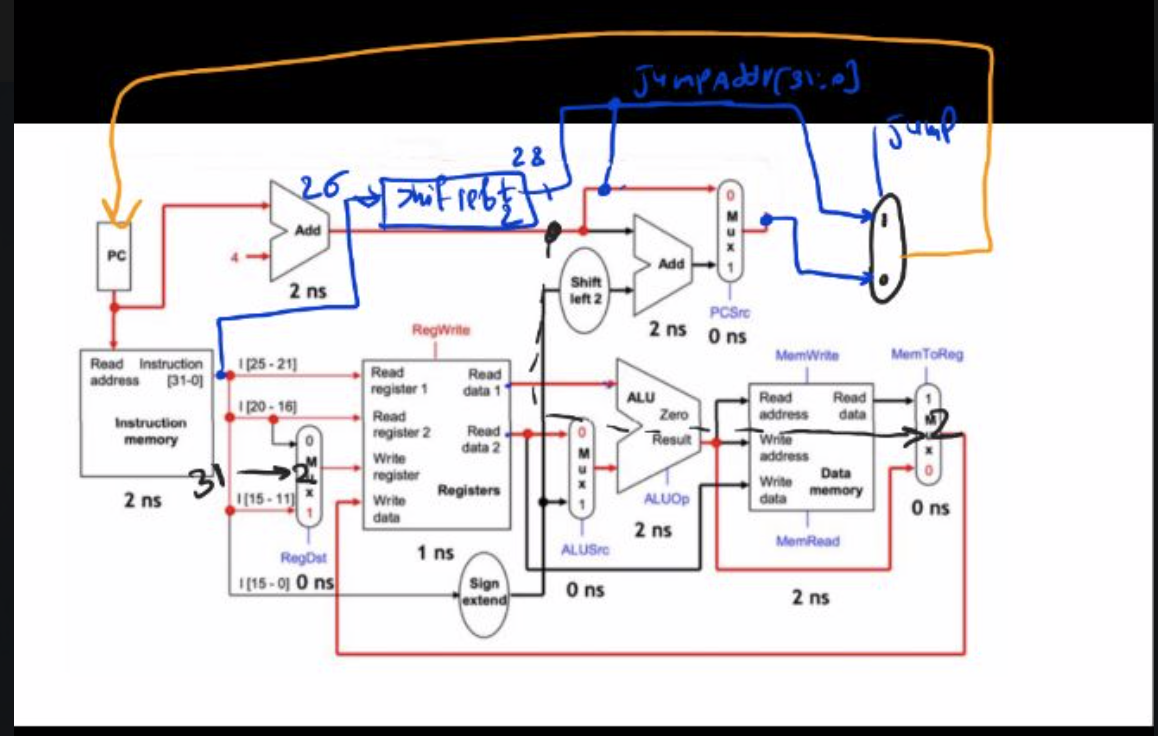
\includegraphics[width=1\textwidth]{jal6}
\end{center}
که مقدار سیگنال های کنترلی به شرح زیر می باشد :‌
 \begin{center}
	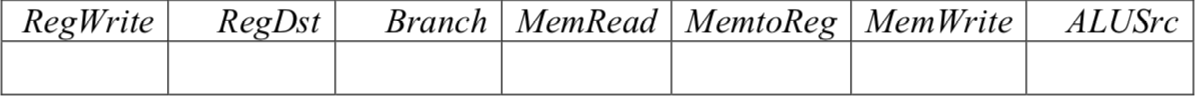
\includegraphics[width=1\textwidth]{beq}
\end{center}
\section*{سوال عملی }
در طراحی این مدار از واحد هایی برای شیفت دادن و همچنین 
\lr{sign extend}
کردن  استفاده شده که جزئیات آن در طراحی آمده است  . 
\\
\textbf{به دلیل این که در صورت سوال گفته نشده که مقدار اولیه 
\lr{PC}
را چند باید در نظر گرفت ، این مقدار 
\textcolor{red}{صفر}
در نظر گرفته شده است  . 
}
\end{document}